\begin{comment}
Template vir elke funksie
    \paragraph{Funksie naam}
			\begin{description}
			    \item{\textbf{Priority}:} %watter prioriteit dit het: Critical, Important of Nic-to-have
			    \item{\textbf{Service Contract}:}% Wat dit doen
			    \item{\textbf{Pre-conditions}:}%wat moet waar wees voor die funksie sy ding kan doen
    			    \begin{itemize}
    			        \item %precondition 1
    			        \item %precondition 2
    			    \end{itemize}
			    \item{\textbf{Post-conditions}:} % wat moet waar wees na die funksie sy ding gedoen het
    			    \begin{itemize}
    			    \item %post condition 1
    			    \item %post condition2
    			    \end{itemize}
			\end{description}
\end{comment}






\subsection{Website}


	\subsubsection{Scope}
	The website is used by a user to manage his meetings. 
	
	\subsubsection{Functionality}
	
    	\paragraph{Register}
			\begin{description}
			    \item{\textbf{Priority}:} Important
			    \item{\textbf{Service Contract}:} The user enters his name, surname, email address and password. These details are stored in the database on the server and the user is automatically logged in.
			    \item{\textbf{Pre-conditions}:}%wat moet waar wees voor die funksie sy ding kan doen
    			    \begin{itemize}
    			        \item The user must be connected to the Internet.
    			        \item The server must running.
    			    \end{itemize}
			    \item{\textbf{Post-conditions}:} % wat moet waar wees na die funksie sy ding gedoen het
    			    \begin{itemize}
    			    \item The users name, surname, email address and password are stored in the database. 
    			    \item login function is called with the users details.
    			    \item  The action is logged in the database.
    			    \end{itemize}
			\end{description}
	
	\begin{figure}[H]	
 			 \centering
			  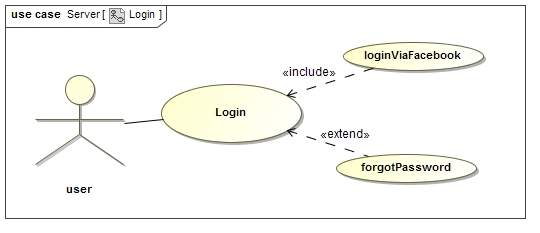
\includegraphics[width=12cm]{LoginUseCase}
		 	 \caption{A Use Case Diagram of the Login services}
		\end{figure}
    	\paragraph{Log in}
			\begin{description}
			    \item{\textbf{Priority}:} Important
			    \item{\textbf{Service Contract}:}The user types his email address and password to enter the website
			    \item{\textbf{Pre-conditions}:}%wat moet waar wees voor die funksie sy ding kan doen
    			    \begin{itemize}
    			        \item The browser must be connected to the Internet.
    			        \item The server must running.
    			        \item The user must be registered.
    			        \item The password must be correct.
    			    \end{itemize}
			    \item{\textbf{Post-conditions}:}
    			    \begin{itemize}
    			    \item The user becomes the current user on the website session.%sê beter
    			    \item The user is on his home page.
    			    \item  The action is logged in the database.
    			    
    			    \end{itemize}
			\end{description}
			
    	\paragraph{Log out}
			\begin{description}
			    \item{\textbf{Priority}:} Important
			    \item{\textbf{Service Contract}:} The user clicks on a button and the user is logged out of his account. 
			    \item{\textbf{Pre-conditions}:}
    			    \begin{itemize}
    			        \item The browser must be connected to the Internet.
    			        \item The server must running. 	
    			        \item The user has to be logged in. 
    			    \end{itemize}
			    \item{\textbf{Post-conditions}:} 
    			    \begin{itemize}
    			      \item The user is logged out.
    			      \item The current user on the session becomes null.
    			      \item The browser is redirected to the log in page 
    			      \item  The action is logged in the database.
    			    \end{itemize}
			\end{description}
			
    	\paragraph{Reset password}
			\begin{description}
			    \item{\textbf{Priority}:} Nice to Have
			    \item{\textbf{Service Contract}:} The user can reset a forgotten password. The function is available on the log in page. 
			    \item{\textbf{Pre-conditions}:}
    			    \begin{itemize}
    			        \item The browser must be connected to the Internet.
    			        \item The server must running. 	
    			        \item The user should not be logged in. 
    			        \item The user has to provide an email address.
    			    \end{itemize}
			    \item{\textbf{Post-conditions}:} 
    			    \begin{itemize}
    			      \item An email is send to the users email address with a link to the reset password web page. The user has to open it.
    			      \item On the reset password page, the user enters the password twice.
    			      \item The users password is changed in the database.
    			      \item The user is redirected to the log in page.
    			      \item  The action is logged in the database.
    			    \end{itemize}
			\end{description}
							
			
    	\paragraph{Create Meeting}
			\begin{description}
			    \item{\textbf{Priority}:} Critical
			    \item{\textbf{Service Contract}:} The user schedules a meeting by entering the title, description, meeting room, time and date.
			    \item{\textbf{Pre-conditions}:}
    			    \begin{itemize}
    			        \item The browser must be connected to the Internet.
    			        \item The server must running.    		  
    			        \item The user has to be logged in. 
    			        \item The meeting title, meeting room, date and time are required fields.
    			    \end{itemize}
			    \item{\textbf{Post-conditions}:} 
    			    \begin{itemize}
    			      \item The meeting and its details are stored in the database.
    			      \item The meeting is  added to the users list of meetings on the database. 
    			      \item The update meeting, invite person and remove meeting functions are available. 
    			      \item  The action is logged in the database. 
    			    \end{itemize}
			\end{description}
			
    	\paragraph{Invite Person}
			\begin{description}
			    \item{\textbf{Priority}:} Critical
			    \item{\textbf{Service Contract}:} The user invites a person to a specific meeting. This function is called for every person being invited.
			    \item{\textbf{Pre-conditions}:}
    			    \begin{itemize}
    			        \item The browser must be connected to the Internet.
    			        \item The server must running.	        
    			        \item The user has to be logged in. 
    			        \item The meeting has to be specified.
    			        \item The required fields for the person being invited are: the name, surname and email address.
    			    \end{itemize}
			    \item{\textbf{Post-conditions}:} 
    			    \begin{itemize}
    			      \item If the person does not yet exist in the database he is added to the database.
    			      \item The person is added to the meetings list of invited people. 
    			      \item An email is send to the person to notify him of the meeting.
    			      \item The action is logged in the database.
    			    \end{itemize}
			\end{description}	
			
    	\paragraph{Remove Person}
			\begin{description}
			    \item{\textbf{Priority}:} Important
			    \item{\textbf{Service Contract}:} The user removes a person from the list of invited people of a specified meeting.
			    \item{\textbf{Pre-conditions}:}
    			    \begin{itemize}
    			        \item The browser must be connected to the Internet.
    			        \item The server must running.    	       
    			        \item The user has to be logged in. 
    			        \item The meeting has to be specified.
    			        \item The person has to be specified.
    			        \item The person has to exist in the meetings list of invited people.
    			        \item The user has to confirm the action.
    			    \end{itemize}
			    \item{\textbf{Post-conditions}:} 
    			    \begin{itemize}
    			      \item The person is removed from the list of invited people of the meeting.
    			      \item The person is not removed from the database. 
    			      \item An email is send to the person to notify him that he has been removed from the list.
    			      \item The action is logged in the database.
    			    \end{itemize}
			\end{description}	
			
    	\paragraph{Update Meeting}
			\begin{description}
			    \item{\textbf{Priority}:} Important
			    \item{\textbf{Service Contract}:} The user can update any of the specified meetings fields.
			    \item{\textbf{Pre-conditions}:}
    			    \begin{itemize}
    			        \item The browser must be connected to the Internet.
    			        \item The server must running.
    			        \item The user has to be logged in. 
    			        \item The meeting has to be specified.
    			    \end{itemize}
			    \item{\textbf{Post-conditions}:} 
    			    \begin{itemize}
    			      \item The change is made to the meeting in the database.
    			      \item The action is logged in the database.
    			    \end{itemize}
			\end{description}	
	    
	    \paragraph{Remove Meeting}
			\begin{description}
			    \item{\textbf{Priority}:} Important %watter prioriteit dit het: Critical, Important of Nic-to-have
			    \item{\textbf{Service Contract}:} The specified meeting is logically removed from the database.% Wat dit doen
			    \item{\textbf{Pre-conditions}:}%wat moet waar wees voor die funksie sy ding kan doen
    			    \begin{itemize}
    			        \item The browser must be connected to the Internet.
    			        \item The server must running.
    			        \item The user has to be logged in. 
    			        \item The meeting has to be specified.
    			    \end{itemize}
			    \item{\textbf{Post-conditions}:} % wat moet waar wees na die funksie sy ding gedoen het
    			    \begin{itemize}
    			    \item All the invited people are notified via email.
    			    \item The meeting is no on the owners list of meetings.
    			    \item The meeting is no longer on the invited peoples list of meetings.
    			    \item The action is logged in the databases.
    			    \end{itemize}
			\end{description}
			
					
							
			
